\section{Технологическая часть}

\subsection{Средства реализации}

В качестве системы управления базами данных выбрана  \textbf{PostgreSQL}~\cite{postgresql}, которая обеспечивает надёжность, поддерживает механизмы целостности данных и безопасность на уровне ролей и строк (RLS), что важно для строгого разграничения прав доступа между пользователями. PostgreSQL является одной из самых популярных систем управления базами данных~\cite{DBEnginesRanking}, и у меня есть опыт работы с ней.

Для кэширования данных используется  \textbf{Redis}~\cite{redis}, что помогает повысить производительность и сократить нагрузку на базу данных. Redis является популярным и проверенным решением~\cite{DBEnginesRanking}, и у меня есть опыт работы с ним.

Язык программирования  \textbf{Swift}~\cite{swift} выбран для разработки приложения, поскольку он идеально интегрируется с экосистемой iOS, поддерживает все необходимые инструменты для работы с базой данных и создания графического интерфейса. Также имеется опыт работы с Swift.

Выбраны среды разработки \textbf{Xcode}~\cite{xcode} и \textbf{pgAdmin 4}~\cite{pgadmin4}, так как они предоставляют все необходимые инструменты для создания мобильного приложения и управления базой данных.

\subsection{Реализация базы данных}

Далее представлены реализации спроектированной базы данных: ее сущностей, ограничений целостности данных, ролевой модели и триггеров.

\subsubsection*{Реализация сущностей}

Реализации создания таблиц представлены на листингах~\ref{alg:1}-\ref{alg:12}.

\begin{lstlisting}[label=alg:1, caption=Реализация создания отношения User, captionpos=t]
CREATE TABLE "User" (
	id 				UUID,
	email 			TEXT,
	phone_number 	TEXT,
	"password" 		TEXT,
	first_name 		TEXT,
	last_name 		TEXT,
	gender 			TEXT,
	birth_date 		DATE
);
\end{lstlisting}

\begin{lstlisting}[label=alg:2, caption=Реализация создания отношения UserRole, captionpos=t]
CREATE TABLE "UserRole" (
	id			UUID,
	user_id		UUID,
	"role" 		TEXT
);
\end{lstlisting}

\begin{lstlisting}[label=alg:3, caption=Реализация создания отношения Trainer, captionpos=t]
CREATE TABLE "Trainer" (
	id 				UUID,
	user_id			UUID,
	description 	TEXT
);
\end{lstlisting}

\begin{lstlisting}[label=alg:13, caption=Реализация создания отношения Specialization, captionpos=t]
CREATE TABLE "Specialization" (
	id	 	UUID,
	name 	TEXT
);
\end{lstlisting}

\begin{lstlisting}[label=alg:4, caption=Реализация создания отношения TrainerSpecialization, captionpos=t]
-- Специализация тренера
CREATE TABLE "TrainerSpecialization" (
	id 					UUID,
	trainer_id			UUID,
	specialization_id	UUID,
	years				INT
);
\end{lstlisting}

\begin{lstlisting}[label=alg:5, caption=Реализация создания отношения MembershipType, captionpos=t]
CREATE TABLE "MembershipType" (
	id 			UUID,
	name 		TEXT,
	price 		NUMERIC,
	sessions	INT,
	days		INT
);
\end{lstlisting}

\begin{lstlisting}[label=alg:6, caption=Реализация создания отношения TrainingRoom, captionpos=t]
CREATE TABLE "TrainingRoom" (
	id			UUID,
	name	 	TEXT,
	capacity 	INT
);
\end{lstlisting}

\begin{lstlisting}[label=alg:7, caption=Реализация создания отношения Order, captionpos=t]
CREATE TABLE "Order" (
	id 			UUID,
	user_id		UUID,
	"date" 		TIMESTAMP,
	total_price NUMERIC
);
\end{lstlisting}

\begin{lstlisting}[label=alg:8, caption=Реализация создания отношения OrderItem, captionpos=t]
CREATE TABLE "OrderItem" (
	id 					UUID,
	order_id 			UUID,
	membership_type_id 	UUID
);
\end{lstlisting}

\begin{lstlisting}[label=alg:9, caption=Реализация создания отношения Payment, captionpos=t]
CREATE TABLE "Payment" (
	id				UUID,
	order_id		UUID,
	transaction_id 	TEXT,
	"date" 			TIMESTAMP,
	"method" 		TEXT,
	gateway 		TEXT,
	status 			TEXT
);
\end{lstlisting}

\begin{lstlisting}[label=alg:10, caption=Реализация создания отношенияMembership, captionpos=t]
CREATE TABLE "Membership" (
	id 					UUID,
	user_id				UUID,
	order_id			UUID,
	membership_type_id	UUID,
	start_date			DATE,
	end_date			DATE,
	available_sessions	INT
);
\end{lstlisting}

\begin{lstlisting}[label=alg:11, caption=Реализация создания отношения Training, captionpos=t]
CREATE TABLE "Training" (
	id 					UUID,
	specialization_id	UUID,
	room_id				UUID,
	trainer_id			UUID,
	"date"				TIMESTAMP
);
\end{lstlisting}

\begin{lstlisting}[label=alg:12, caption=Реализация создания отношения Attendance, captionpos=t]
	CREATE TABLE "Attendance" (
	id 				UUID,
	membership_id	UUID,
	training_id		UUID,
	status			TEXT
);
\end{lstlisting}


\subsubsection*{Реализация ограничений целостности данных}

Реализации ограничений целостности данных таблиц представлены на листингах~\ref{alg:14}-\ref{alg:26}.

\begin{lstlisting}[label=alg:14, caption=Реализация  ограничений целостности данных отношения User, captionpos=t]
ALTER TABLE "User"
	ADD CONSTRAINT "pk:user.id" PRIMARY KEY (id),
	ALTER COLUMN id SET DEFAULT gen_random_uuid(),
	ADD CONSTRAINT "chk:user.email:notnull" CHECK (email IS NOT NULL),
	ADD CONSTRAINT "chk:user.email:length" CHECK (length(email) < 128),
	ADD CONSTRAINT "chk:user.email:regexp" CHECK (
		email ~ '^[A-Za-z0-9._%-]+@[A-Za-z0-9.-]+[.][A-Za-z]+$'),
	ADD CONSTRAINT "uq:user.email" UNIQUE (email),
	ADD CONSTRAINT "chk:user.phone_number:notnull" CHECK (
		phone_number IS NOT NULL),
	ADD CONSTRAINT "chk:user.phone_number:length" CHECK (
		length(phone_number) < 32),
	ADD CONSTRAINT "chk:user.phone_number:regexp" CHECK (
		phone_number ~ '^\+\d{10,15}$'),
	ADD CONSTRAINT "uq:user.phone_number" UNIQUE (phone_number),
	ADD CONSTRAINT "chk:user.password:notnull" CHECK (
		"password" IS NOT NULL),
	ADD CONSTRAINT "chk:user.first_name:notnull" CHECK (
		first_name IS NOT NULL),
	ADD CONSTRAINT "chk:user.first_name:length" CHECK (
		length(first_name) < 128),
	ADD CONSTRAINT "chk:user.first_name:regexp" CHECK (
		first_name ~ '^([a-zA-Zа-яА-ЯёЁ]+(?:-[a-zA-Zа-яА-ЯёЁ]+)?)$'),
	ADD CONSTRAINT "chk:user.last_name:notnull" CHECK (
		last_name IS NOT NULL),
	ADD CONSTRAINT "chk:user.last_name:length" CHECK (
		length(last_name) < 128),
	ADD CONSTRAINT "chk:user.last_name:regexp" CHECK (
		last_name ~ '^([a-zA-Zа-яА-ЯёЁ]+(?:-[a-zA-Zа-яА-ЯёЁ]+)?)$'),
	ADD CONSTRAINT "chk:user.gender:notnull" CHECK (gender IS NOT NULL),
	ADD CONSTRAINT "chk:user.gender:length" CHECK (length(gender) < 32),
	ADD CONSTRAINT "chk:user.gender:regexp" CHECK (
		gender IN ('мужской', 'женский')),
	ADD CONSTRAINT "chk:user.birth_date:notnull" CHECK (
		birth_date IS NOT NULL),
	ADD CONSTRAINT "chk:user.birth_date" CHECK (
		birth_date BETWEEN 
			CURRENT_DATE - INTERVAL '120 years' AND 
			CURRENT_DATE - INTERVAL '14 years'
	);
\end{lstlisting}

\begin{lstlisting}[label=alg:15, caption=Реализация  ограничений целостности данных отношения UserRole, captionpos=t]
ALTER TABLE "UserRole"
	ADD CONSTRAINT "pk:user_role.id" PRIMARY KEY (id),
	ALTER COLUMN id SET DEFAULT gen_random_uuid(),
	ADD CONSTRAINT "fk:user_role.user_id" FOREIGN KEY (user_id) 
		REFERENCES "User"(id) ON DELETE CASCADE,
	ADD CONSTRAINT "uq:user_role.user_id" UNIQUE (user_id),
	ADD CONSTRAINT "chk:user_role.role:notnull" CHECK ("role" IS NOT NULL),
	ADD CONSTRAINT "chk:user_role.role:length" CHECK (length("role") < 32),
	ADD CONSTRAINT "chk:user_role.role:regexp" CHECK (
		"role" IN ('клиент', 'тренер', 'администратор')
	);
\end{lstlisting}

\begin{lstlisting}[label=alg:16, caption=Реализация  ограничений целостности данных отношения Trainer, captionpos=t]
ALTER TABLE "Trainer"
	ADD CONSTRAINT "pk:trainer.id" PRIMARY KEY (id),
	ALTER COLUMN id SET DEFAULT gen_random_uuid(),
	ADD CONSTRAINT "fk:trainer.user_id" FOREIGN KEY (user_id) 
		REFERENCES "User"(id) ON DELETE CASCADE,
	ADD CONSTRAINT "uq:trainer.user_id" UNIQUE (user_id),
	ALTER COLUMN "description" SET DEFAULT 'Нет описания.',
	ADD CONSTRAINT "chk:trainer.description:notnull" CHECK (
		description IS NOT NULL),
	ADD CONSTRAINT "chk:trainer.description:length" CHECK (
		length(description) < 512);
\end{lstlisting}

\begin{lstlisting}[label=alg:17, caption=Реализация  ограничений целостности данных отношения Specialization, captionpos=t]
ALTER TABLE "Specialization"
	ADD CONSTRAINT "pk:specialization.id" PRIMARY KEY (id),
	ALTER COLUMN id SET DEFAULT gen_random_uuid(),
	ADD CONSTRAINT "chk:specialization.name:notnull" CHECK (
		name IS NOT NULL),
	ADD CONSTRAINT "chk:specialization.name:length" CHECK (
		length(name) < 128),
	ADD CONSTRAINT "uq:specialization.name" UNIQUE (name);
\end{lstlisting}

\begin{lstlisting}[label=alg:18, caption=Реализация  ограничений целостности данных отношения TrainerSpecialization, captionpos=t]
ALTER TABLE "TrainerSpecialization"
	ADD CONSTRAINT "pk:trainer_specialization.id" PRIMARY KEY (id),
	ALTER COLUMN id SET DEFAULT gen_random_uuid(),
	ADD CONSTRAINT "fk:trainer_specialization.trainer_id" 
		FOREIGN KEY (trainer_id) REFERENCES "Trainer"(id) ON DELETE CASCADE,
	ADD CONSTRAINT "fk:trainer_specialization.specialization_id" 
		FOREIGN KEY (specialization_id) 
		REFERENCES "Specialization"(id) ON DELETE CASCADE,
	ADD CONSTRAINT "uq:trainer_specialization.trainer+specialization" 
		UNIQUE (trainer_id, specialization_id),
	ALTER COLUMN years SET DEFAULT 0,
	ADD CONSTRAINT "chk:trainer_specialization.years:notnull" CHECK (
		years IS NOT NULL),
	ADD CONSTRAINT "chk:specialization.name:unsigned" CHECK (years >= 0);
\end{lstlisting}

\begin{lstlisting}[label=alg:20, caption=Реализация  ограничений целостности данных отношения TrainingRoom, captionpos=t]
ALTER TABLE "TrainingRoom"
	ADD CONSTRAINT "pk:training_room.id" PRIMARY KEY (id),
	ALTER COLUMN id SET DEFAULT gen_random_uuid(),
	ADD CONSTRAINT "chk:training_room.name:notnull" CHECK (name IS NOT NULL),
	ADD CONSTRAINT "chk:training_room.name:length" CHECK (length(name) < 64),
	ADD CONSTRAINT "uq:training_room.name" UNIQUE (name),
	ADD CONSTRAINT "chk:training_room.capacity:notnull" CHECK (
		capacity IS NOT NULL),
	ADD CONSTRAINT "chk:training_room.capacity" CHECK (capacity > 0);
\end{lstlisting}

\begin{lstlisting}[label=alg:21, caption=Реализация  ограничений целостности данных отношения Order, captionpos=t]
ALTER TABLE "Order"
	ADD CONSTRAINT "pk:order.id" PRIMARY KEY (id),
	ALTER COLUMN id SET DEFAULT gen_random_uuid(),
	ADD CONSTRAINT "fk:order.user_id" FOREIGN KEY (user_id) 
		REFERENCES "User"(id) ON DELETE SET NULL,
	ALTER COLUMN "date" SET DEFAULT CURRENT_TIMESTAMP,
	ADD CONSTRAINT "chk:order.date:notnull" CHECK ("date" IS NOT NULL),
	ALTER COLUMN total_price SET DEFAULT 0.0,
	ADD CONSTRAINT "chk:order.total_price:notnull" CHECK (
		total_price IS NOT NULL),
	ADD CONSTRAINT "chk:order.total_price:unsigned" CHECK (total_price >= 0);
\end{lstlisting}

\begin{lstlisting}[label=alg:22, caption=Реализация  ограничений целостности данных отношения OrderItem, captionpos=t]
ALTER TABLE "OrderItem"
	ADD CONSTRAINT "pk:order_item.id" PRIMARY KEY (id),
	ALTER COLUMN id SET DEFAULT gen_random_uuid(),
	ADD CONSTRAINT "fk:order_item.order_id" FOREIGN KEY (order_id) 
		REFERENCES "Order"(id) ON DELETE CASCADE,
	ADD CONSTRAINT "fk:order_item.membership_type_id" 
		FOREIGN KEY (membership_type_id) 
		REFERENCES "MembershipType"(id) ON DELETE CASCADE;
\end{lstlisting}

\begin{lstlisting}[label=alg:23, caption=Реализация  ограничений целостности данных отношения Payment, captionpos=t]
ALTER TABLE "Payment"
	ADD CONSTRAINT "pk:payment.id" PRIMARY KEY (id),
	ALTER COLUMN id SET DEFAULT gen_random_uuid(),
	ADD CONSTRAINT "fk:payment.order_id" FOREIGN KEY (order_id) 
		REFERENCES "Order"(id) ON DELETE SET NULL,
	ADD CONSTRAINT "chk:payment.transaction_id:notnull" CHECK (
		transaction_id IS NOT NULL),
	ADD CONSTRAINT "chk:payment.transaction_id:length" CHECK (
		length(transaction_id) < 256),
	ADD CONSTRAINT "uq:payment.transaction_id" UNIQUE (transaction_id),
	ALTER COLUMN "date" SET DEFAULT CURRENT_TIMESTAMP,
	ADD CONSTRAINT "chk:payment.date:notnull" CHECK ("date" IS NOT NULL),
	ALTER COLUMN "method" SET DEFAULT 'наличные',
	ADD CONSTRAINT "chk:payment.method:notnull" CHECK ("method" IS NOT NULL),
	ADD CONSTRAINT "chk:payment.method:length" CHECK (length("method") < 64),
	ADD CONSTRAINT "chk:payment.method:regexp" CHECK (
		"method" IN ('наличные', 'кредитная карта', 'банковский перевод')),
	ALTER COLUMN "gateway" SET DEFAULT NULL,
	ADD CONSTRAINT "chk:payment.gateway:length" CHECK (
		length("gateway") < 64),
	ALTER COLUMN "status" SET DEFAULT 'ожидает',
	ADD CONSTRAINT "chk:payment.status:notnull" CHECK ("status" IS NOT NULL),
	ADD CONSTRAINT "chk:payment.status:length" CHECK (length("status") < 64),
	ADD CONSTRAINT "chk:payment.status" CHECK (
		status IN ('ожидает', 'оплачен', 'отменен'));
\end{lstlisting}

\begin{lstlisting}[label=alg:19, caption=Реализация  ограничений целостности данных отношения MembershipType, captionpos=t]
	ALTER TABLE "MembershipType"
	ADD CONSTRAINT "pk:membership_type.id" PRIMARY KEY (id),
	ALTER COLUMN id SET DEFAULT gen_random_uuid(),
	ADD CONSTRAINT "chk:membership_type.name:notnull" CHECK (
	name IS NOT NULL),
	ADD CONSTRAINT "chk:membership_type.name:length" CHECK (
	length(name) < 128),
	ADD CONSTRAINT "uq:membership_type.name" UNIQUE (name),
	ALTER COLUMN price SET DEFAULT 0.0,
	ADD CONSTRAINT "chk:membership_type.price:notnull" CHECK (
	price IS NOT NULL),
	ADD CONSTRAINT "chk:membership_type.price:unsigned" CHECK (price >= 0.0),
	ALTER COLUMN sessions SET DEFAULT 1,
	ADD CONSTRAINT "chk:membership_type.sessions:notnull" CHECK (
	sessions IS NOT NULL),
	ADD CONSTRAINT "chk:membership_type.sessions:unsigned" CHECK (
	sessions > 0),
	ALTER COLUMN days SET DEFAULT 1,
	ADD CONSTRAINT "chk:membership_type.days:notnull" CHECK (
	days IS NOT NULL),
	ADD CONSTRAINT "chk:membership_type.days:unsigned" CHECK (days > 0);
\end{lstlisting}

\begin{lstlisting}[label=alg:25, caption=Реализация  ограничений целостности данных отношения Training, captionpos=t]
	ALTER TABLE "Training"
	ADD CONSTRAINT "pk:training.id" PRIMARY KEY (id),
	ALTER COLUMN id SET DEFAULT gen_random_uuid(),
	ADD CONSTRAINT "fk:training.specialization_id" 
	FOREIGN KEY (specialization_id) 
	REFERENCES "Specialization"(id) ON DELETE SET NULL,
	ADD CONSTRAINT "fk:training.room_id" FOREIGN KEY (room_id) 
	REFERENCES "TrainingRoom"(id) ON DELETE SET NULL,
	ADD CONSTRAINT "fk:training.trainer_id" FOREIGN KEY (trainer_id) 
	REFERENCES "Trainer"(id) ON DELETE SET NULL,
	ALTER COLUMN "date" SET DEFAULT CURRENT_TIMESTAMP,
	ADD CONSTRAINT "chk:training.date:notnull" CHECK ("date" IS NOT NULL);
\end{lstlisting}

\begin{lstlisting}[label=alg:24, caption=Реализация  ограничений целостности данных отношения Membership, captionpos=t]
ALTER TABLE "Membership"
	ADD CONSTRAINT "pk:membership.id" PRIMARY KEY (id),
	ALTER COLUMN id SET DEFAULT gen_random_uuid(),
	ADD CONSTRAINT "fk:membership.user_id" FOREIGN KEY (user_id) 
		REFERENCES "User"(id) ON DELETE CASCADE,
	ADD CONSTRAINT "fk:membership.order_id" FOREIGN KEY (order_id) 
		REFERENCES "Order"(id) ON DELETE SET NULL,
	ADD CONSTRAINT "fk:membership.membership_type_id" 
		FOREIGN KEY (membership_type_id) 
		REFERENCES "MembershipType"(id) ON DELETE SET NULL,
	ALTER COLUMN start_date SET DEFAULT NULL,
	ALTER COLUMN end_date SET DEFAULT NULL,
	ADD CONSTRAINT "chk:membership.dates:order" CHECK(
		(start_date IS NULL AND end_date IS NULL) OR (start_date IS NOT NULL 
		AND end_date IS NOT NULL AND start_date <= end_date)),
	ADD CONSTRAINT "uq:membership.membership_type+user"
		UNIQUE(membership_type_id, user_id),
	ALTER COLUMN available_sessions SET DEFAULT 0,
	ADD CONSTRAINT "chk:membership.available_sessions:notnull" CHECK (
		available_sessions IS NOT NULL),
	ADD CONSTRAINT "chk:membership.available_sessions:unsigned" CHECK (
		available_sessions >= 0);
\end{lstlisting}

\begin{lstlisting}[label=alg:26, caption=Реализация  ограничений целостности данных отношения Attendance, captionpos=t]
ALTER TABLE "Attendance"
	ADD CONSTRAINT "pk:attendance.id" PRIMARY KEY (id),
	ALTER COLUMN id SET DEFAULT gen_random_uuid(),
	ADD CONSTRAINT "fk:attendance.membership_id" FOREIGN KEY (membership_id) 
		REFERENCES "Membership"(id) ON DELETE CASCADE,
	ADD CONSTRAINT "fk:attendance.training_id" FOREIGN KEY (training_id) 
		REFERENCES "Training"(id) ON DELETE SET NULL,
	ADD CONSTRAINT "uq:attendance.membership+training" 
		UNIQUE (membership_id, training_id),
	ALTER COLUMN status SET DEFAULT 'ожидает',
	ADD CONSTRAINT "chk:attendance.status:notnull" CHECK (
		status IS NOT NULL),
	ADD CONSTRAINT "chk:attendance.status:length" CHECK (
		length(status) < 64),
	ADD CONSTRAINT "chk:attendance.status:regexp" CHECK (
		status IN ('посетил', 'отсутствовал', 'ожидает'));
\end{lstlisting}

\subsubsection{Реализация триггеров}

Реализации триггеров для: автоматического обновления количества доступных занятий после посещения тренировки, записи на тренировку с учетом проверки количества доступных мест, создания абонемента или продления его после успешного платежа -- представлены на листингах~\ref{alg:27},~\ref{alg:28} и~\ref{alg:29} соответственно.

\begin{lstlisting}[label=alg:27, caption=Реализация триггера для автоматического обновления количества доступных занятий после посещения тренировки, captionpos=t]
CREATE OR REPLACE FUNCTION update_available_sessions()
RETURNS TRIGGER AS $$
BEGIN
	IF (NEW.status = 'посетил' OR NEW.status = 'отсутствовал') 
		AND (OLD.status <> 'посетил' AND OLD.status <> 'отсутствовал') 
	THEN
		UPDATE "Membership"
		SET available_sessions = available_sessions - 1
		WHERE id = NEW.membership_id;
	ELSIF (NEW.status = 'ожидает') 
		AND (OLD.status = 'посетил' OR OLD.status = 'отсутствовал') 
	THEN
		UPDATE "Membership"
		SET available_sessions = available_sessions + 1
		WHERE id = NEW.membership_id;
	END IF;
	RETURN NEW;
END;
$$ LANGUAGE plpgsql;
CREATE OR REPLACE TRIGGER attendance_status_update
AFTER UPDATE OF status ON "Attendance"
FOR EACH ROW
EXECUTE FUNCTION update_available_sessions();
\end{lstlisting}

\begin{lstlisting}[label=alg:28, caption=Реализация триггера для записи на тренировку с учетом проверки количества доступных мест, captionpos=t]
CREATE OR REPLACE FUNCTION check_room_capacity()
RETURNS TRIGGER AS $$
BEGIN
	IF (TG_OP = 'INSERT') OR (TG_OP = 'UPDATE' AND NEW.training_id IS DISTINCT FROM OLD.training_id) 
	THEN
		IF (SELECT COUNT(*) FROM "Attendance" WHERE training_id = NEW.training_id) >= (SELECT capacity FROM "TrainingRoom" WHERE id = (SELECT room_id  FROM public.training WHERE id = NEW.training_id))
		THEN RAISE EXCEPTION 'Тренировка уже заполнена';
		END IF;
	END IF;
	RETURN NEW;
END; $$ LANGUAGE plpgsql;
CREATE OR REPLACE TRIGGER check_room_capacity_trigger
BEFORE INSERT ON "Attendance" FOR EACH ROW
EXECUTE FUNCTION check_room_capacity();
\end{lstlisting}

\begin{lstlisting}[label=alg:29, caption=Реализация триггера для создания абонемента или продления его после успешного платежа , captionpos=t]
CREATE OR REPLACE FUNCTION create_membership_after_payment()
RETURNS TRIGGER AS $$
DECLARE item RECORD;
BEGIN
	IF (TG_OP = 'INSERT' AND NEW.status = 'оплачено') OR (TG_OP = 'UPDATE' AND NEW.status = 'оплачено' AND OLD.status IS DISTINCT FROM 'оплачено') 
	THEN
		FOR item IN
			SELECT oi.membership_type_id, o.user_id, mt.duration_days, mt.number_of_sessions
			FROM "OrderItem" oi
			JOIN "Order" o ON o.id = oi.order_id
			JOIN "MembershipType" mt ON mt.id = oi.membership_type_id
			WHERE o.id = NEW.order_id
		LOOP
			IF EXISTS (SELECT 1 FROM "Membership" WHERE user_id = item.user_id AND membership_type_id = item.membership_type_id) 
			THEN -- обновление
				UPDATE "Membership"
				SET 
				end_date = CURRENT_DATE + INTERVAL '1 day' * item.duration_days,
				available_sessions = available_sessions + item.number_of_sessions,
				order_id = NEW.order_id
				WHERE user_id = item.user_id
				AND membership_type_id = item.membership_type_id;
			ELSE
				INSERT INTO public.membership (id, user_id, membership_type_id, order_id,
				start_date, end_date, available_sessions)
				VALUES (gen_random_uuid(), item.user_id, item.membership_type_id, NEW.order_id, CURRENT_DATE, CURRENT_DATE + INTERVAL '1 day' * item.duration_days, item.number_of_sessions);
			END IF;
		END LOOP;
	END IF;
	RETURN NEW;
END;
$$ LANGUAGE plpgsql;
CREATE OR REPLACE TRIGGER create_membership_after_payment_trigger
AFTER INSERT OR UPDATE ON "Payment" FOR EACH ROW
EXECUTE FUNCTION create_membership_after_payment();
\end{lstlisting}

\subsubsection{Создание ролевой модели}

Реализация ролевой модели представлена на листингах~\ref{alg:30},~\ref{alg:31} и~\ref{alg:32}.

\begin{lstlisting}[label=alg:30, caption=Реализация роли Guest (гость), captionpos=t]
CREATE ROLE guest WITH LOGIN;
GRANT EXECUTE ON FUNCTION register_user(
	UUID, TEXT, TEXT, TEXT, TEXT, TEXT, DATE, TEXT
) TO guest;
GRANT EXECUTE ON FUNCTION login_user(TEXT, TEXT) TO guest;
\end{lstlisting}

\begin{lstlisting}[label=alg:31, caption=Реализация роли Admin (администратор), captionpos=t]
CREATE ROLE admin WITH LOGIN PASSWORD 'admin' SUPERUSER BYPASSRLS;
GRANT ALL PRIVILEGES ON ALL TABLES IN SCHEMA public TO admin;
\end{lstlisting}

\begin{lstlisting}[label=alg:32, caption=Реализация ролей Client (клиент) и Trainer (тренер), captionpos=t]
CREATE ROLE client WITH LOGIN PASSWORD 'client';
CREATE ROLE trainer WITH LOGIN PASSWORD 'trainer';
GRANT client TO trainer;
GRANT ALL ON "User" TO client;
GRANT ALL ON "User" TO trainer;
ALTER TABLE "User" ENABLE ROW LEVEL SECURITY;
CREATE POLICY personal_client_trainer_user_policy ON "User" FOR ALL TO client, trainer USING (id = current_user_id());
CREATE POLICY public_client_trainer_user_policy ON "User" FOR SELECT TO client, trainer USING (TRUE);
GRANT ALL ON "Trainer" TO client;
GRANT ALL ON "Trainer" TO trainer;
ALTER TABLE "Trainer" ENABLE ROW LEVEL SECURITY;
CREATE POLICY public_client_trainer_trainer_policy ON "Trainer" FOR SELECT TO client, trainer USING (TRUE);
CREATE POLICY personal_trainer_trainer_policy ON "Trainer" FOR ALL TO trainer USING (user_id = current_user_id());
GRANT ALL ON "Membership" TO client;
GRANT ALL ON "Membership" TO trainer;
ALTER TABLE "Membership" ENABLE ROW LEVEL SECURITY;
CREATE POLICY client_trainer_membership_policy ON "Membership" FOR ALL TO client, trainer USING (user_id = current_user_id());
CREATE POLICY trainer_membership_policy ON "Membership" FOR SELECT TO trainer USING (TRUE);
GRANT ALL ON "Order" TO client;
GRANT ALL ON "Order" TO trainer;
ALTER TABLE "Order" ENABLE ROW LEVEL SECURITY;
CREATE POLICY client_trainer_order_policy ON "Order" FOR ALL TO client, trainer USING (user_id = current_user_id());
GRANT ALL ON "OrderItem" TO client;
GRANT ALL ON "OrderItem" TO trainer;
ALTER TABLE "OrderItem" ENABLE ROW LEVEL SECURITY;
CREATE POLICY client_trainer_order_item_policy ON "OrderItem" FOR ALL TO client, trainer USING ( order_id IN (
	SELECT id FROM "Order" WHERE user_id = current_user_id()));
GRANT ALL ON "Payment" TO client;
GRANT ALL ON "Payment" TO trainer;
ALTER TABLE "Payment" ENABLE ROW LEVEL SECURITY;
CREATE POLICY client_trainer_payment_policy ON "Payment" FOR ALL TO client, trainer USING ( order_id IN (
	SELECT id  FROM "Order" WHERE user_id = current_user_id()));
GRANT ALL ON "Attendance" TO client;
GRANT ALL ON "Attendance" TO trainer;
ALTER TABLE "Attendance" ENABLE ROW LEVEL SECURITY;
CREATE POLICY client_trainer_attendance_policy ON "Attendance" FOR ALL TO client, trainer USING ( membership_id IN (
	SELECT id  FROM "Membership" WHERE user_id = current_user_id()));
CREATE POLICY trainer_attendance_policy  ON "Attendance" FOR ALL TO trainer USING (training_id IN (
	SELECT id  FROM "Training" WHERE trainer_id = (
		SELECT id FROM "Trainer" WHERE user_id = current_user_id())));
GRANT SELECT ON "Specialization" TO client;
GRANT SELECT ON "Specialization" TO trainer;
GRANT SELECT ON "TrainerSpecialization" TO client;
GRANT SELECT ON "TrainerSpecialization" TO trainer;
GRANT ALL ON "Training" TO trainer;
GRANT ALL ON "Training" TO client;
ALTER TABLE "Training" ENABLE ROW LEVEL SECURITY;
CREATE POLICY client_training_select_policy ON "Training" FOR SELECT TO client, trainer USING (TRUE);
CREATE POLICY trainer_training_update_policy ON "Training" FOR ALL TO trainer USING ( trainer_id = (
	SELECT id  FROM public.trainer  WHERE user_id = current_user_id()));
GRANT SELECT ON "MembershipType" TO client;
GRANT SELECT ON "MembershipType" TO trainer;
GRANT SELECT ON "TrainingRoom" TO client;
GRANT SELECT ON "TrainingRoom" TO trainer;
\end{lstlisting}

\subsection{Тестирование}

На рисунках~\ref{fig:t1} и~\ref{fig:t2} изображено тестирование триггера для создания абонемент или продления его после успешного платежа.

На рисунках~\ref{fig:t3} и~~\ref{fig:t4} изображено тестирование триггеров для: автоматического обновления количества доступных занятий после посещения тренировки, записи на тренировку с учетом проверки количества доступных мест.

\newpage
\begin{figure}[ht!]
	\begin{center}
		\begin{minipage}[b]{0.5\linewidth}
			\centering
			\rotatebox{90}{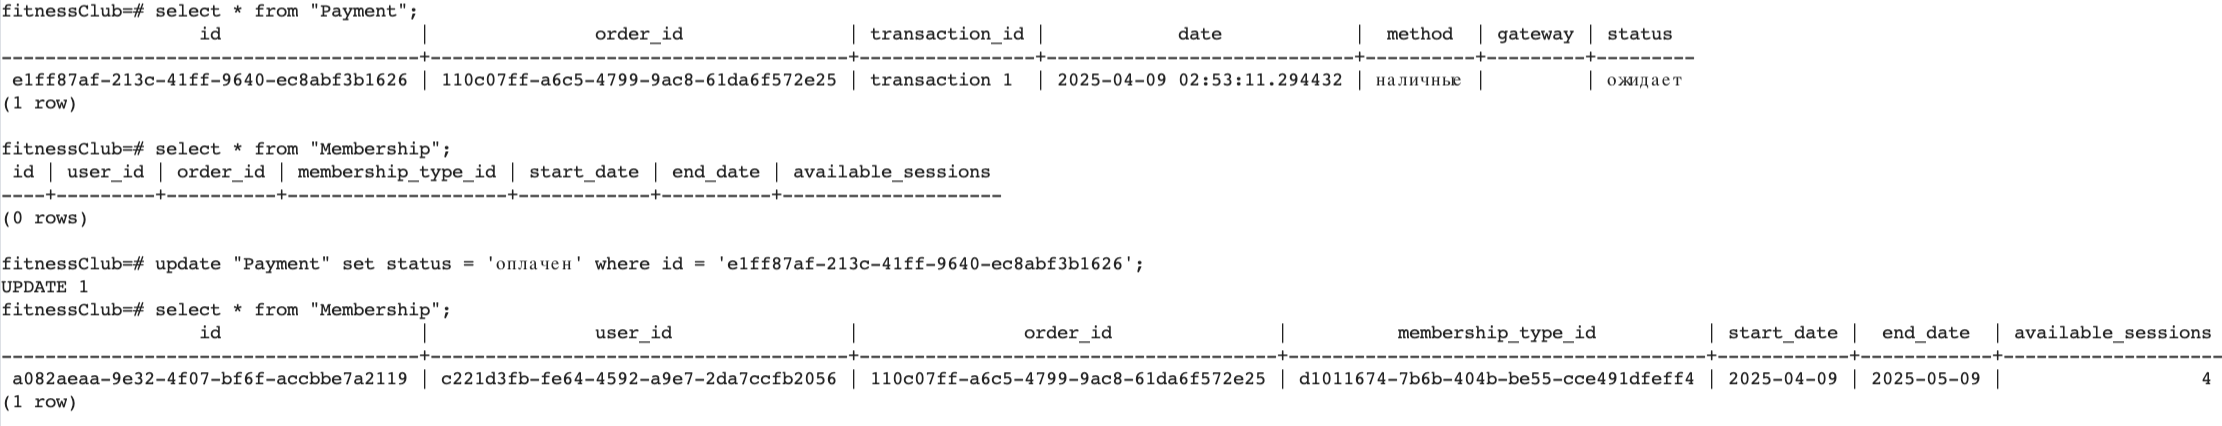
\includegraphics[scale=0.58]{./img/test1.png}}
			\caption{Обновления статуса записи таблицы Payment}
			\label{fig:t1}
		\end{minipage}%
		\begin{minipage}[b]{0.5\linewidth}
			\centering
			\rotatebox{90}{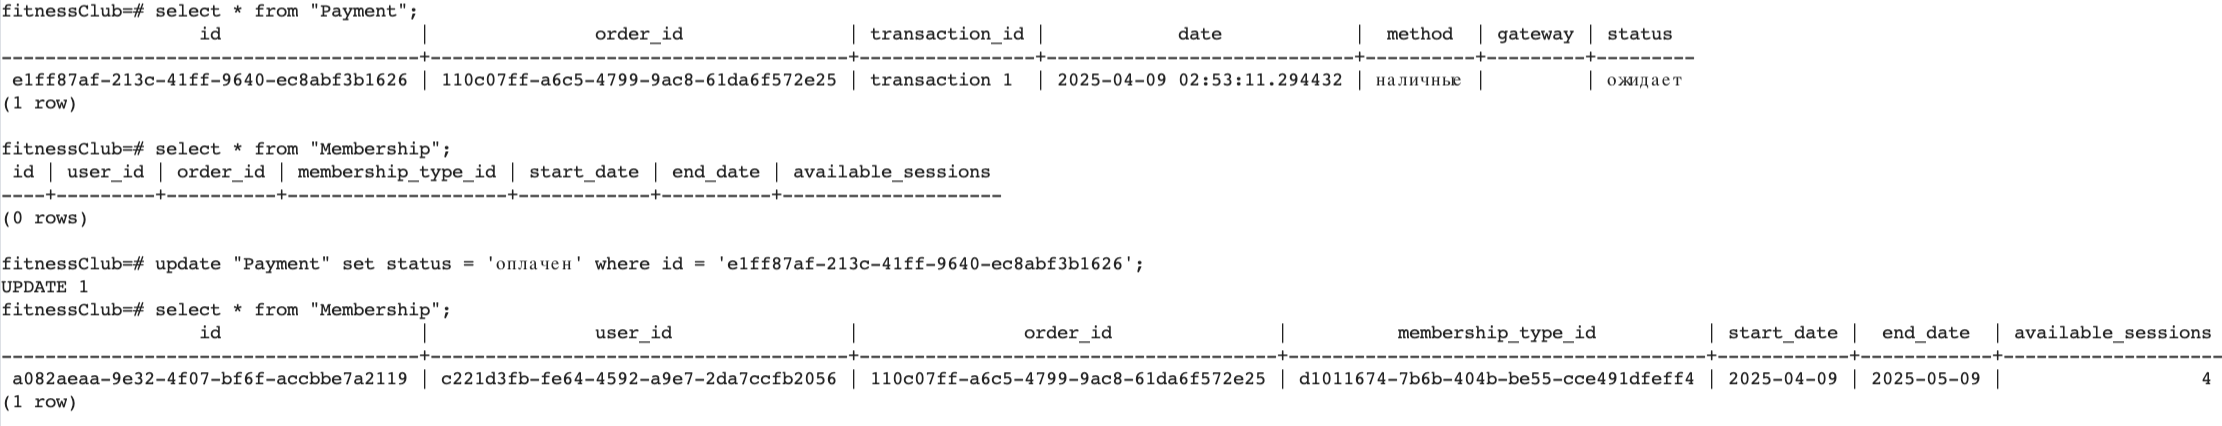
\includegraphics[scale=0.58]{./img/test1.png}}
			\caption{Добавление записи в таблицу Payment}
			\label{fig:t2}
		\end{minipage}
	\end{center}
\end{figure}

\newpage
\begin{figure}[ht!]
	\begin{center}
		\rotatebox{90}{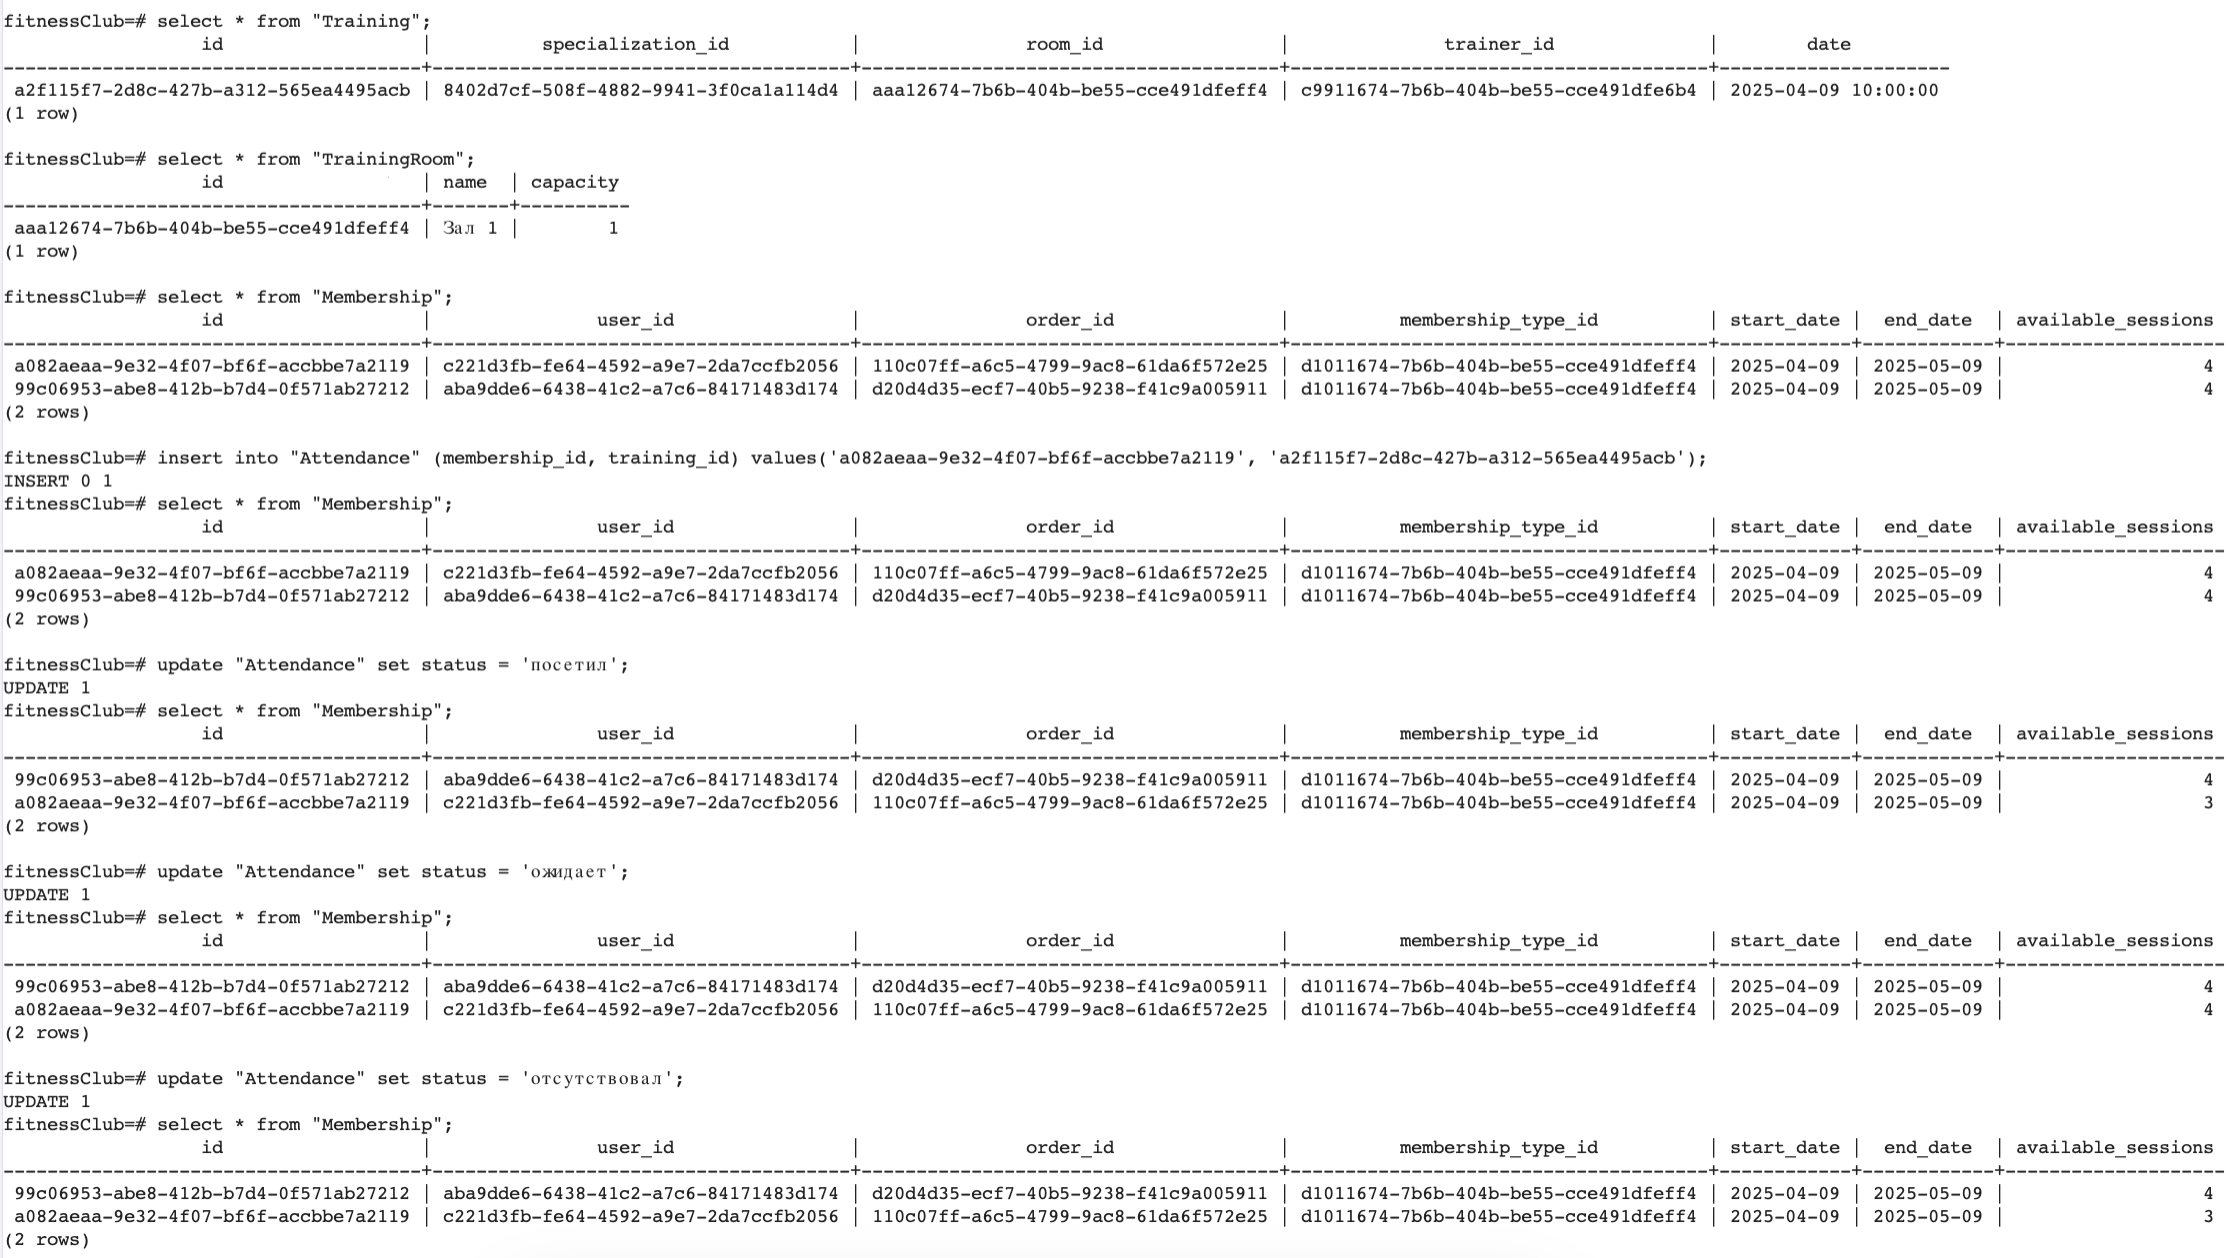
\includegraphics[scale=0.58]{./img/test3.png}}
	\end{center}
	\caption{Добавление записи в таблицу Attendance и обновление ее статуса}
	\label{fig:t3}
\end{figure}

\newpage
\begin{figure}[ht!]
	\begin{center}
		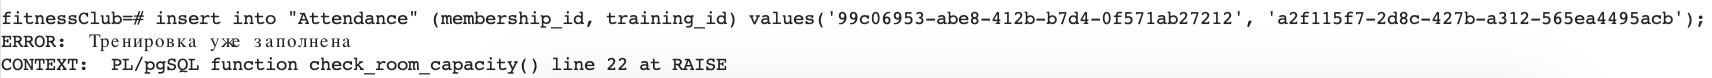
\includegraphics[scale=0.58]{./img/test4.png}
	\end{center}
	\caption{Добавление записи в таблицу Attendance при отсутствии доступных мест на тренировку}
	\label{fig:t4}
\end{figure}

\subsection{Интерфейс для взаимодействая с базой данных}

Для взаимодействия с базой данных реализовано мобильное приложение для платформы iOS. Визуальное представление интерфейса приведено на рисунках~\ref{ios1}-~\ref{ios2} в приложении А. 

\subsection*{Вывод}

В данном разделе представлены выбранные средства реализации, приведены реализации сущностей, ограничений целостности данных, ролевой модели и триггеров. Также описано тестирование триггеров и продемонстрирован интерфейс, обеспечивающий взаимодействие с базой данных.